\chapter{Resultados obtenidos}
\label{resul}
Inicialmente se toma un grafo modelo que se presenta en la figura \ref{Grafomodelo} con su matriz de adyacencia y valores fijos para sus bandits. Se le da libertad al algoritmo a evaluar, que genere aleatoriamente los valores de los bandit en la forma distorsionada que simula la incertidumbre del ejercicio y que decida las rutas a seguir, también, de forma aleatoria.

Los valores de la matriz de adyacencia correspondiente a este grafo se aprecia en el apéndice \ref{run1}, junto con los valores que se dieron a cada uno de sus nodos.

\begin{figure}[h]
  \centering
    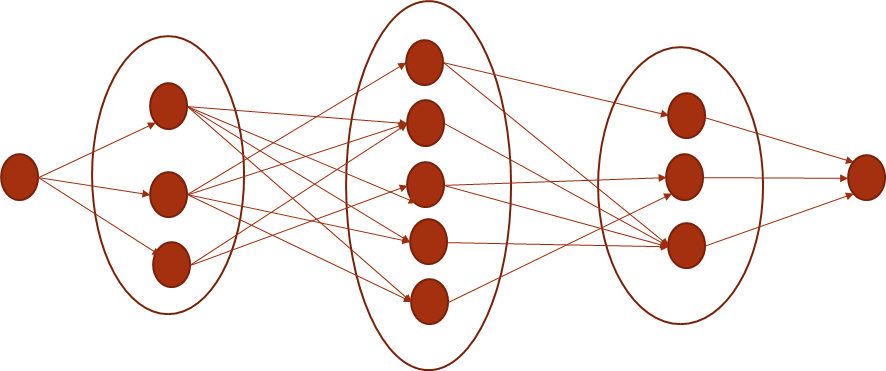
\includegraphics[scale=0.5]{GrafoModelo.png}
  \caption[Grafo Modelo]{Grafo Modelo con 5 etapas y 13 nodos}
  \label{Grafomodelo}
\end{figure}

Las figuras generadas por la aplicación muestran en la curva superior (verde) la ganancia de la mejor ruta probada hasta ese momento, calculada con el valor real de los bandits o medias asignadas a cada uno. Esto se realiza de esta forma para permitir que el software estime la mejor ruta, de un conjunto aleatorio de datos, sin una intervención manual, que equivaldría a una búsqueda exhaustiva.

Seguidamente, en la curva más variable (roja) se presentan las ganancias obtenidas en cada una de las iteraciones por la ruta allí seleccionada, calculada con los valores distorsionados de los bandits, que fueron generados alrededor de las medias reales con desviación estándar de 1. 

Y, por último, en la curva inferior (azul) se muestra el promedio acumulado de estas ganancias, el cual converge a un único valor a través del tiempo y se espera que se acerque al valor real de la mejor ruta, representado en la línea superior.

Se ejecuta el código 10 veces consecutivas para obtener una estimación inicial de su efectividad, cada vez con 999 iteraciones.

Los resultados obtenidos entregan el vector de nodos de las L etapas que ofrece la mayor ganancia, como es [0,2,4,11,12], para los dos modelos, que, en este caso, se puede verificar manualmente.

Como en otras oportunidades, se obtiene solo un porcentaje de ejecuciones que llevan a la respuesta correcta siguiendo el procedimiento de generación aproximada de la matriz de transición de probabilidades, como se puede apreciar en las figuras \ref{graf1}, \ref{graf2}, \ref{graf3}, \ref{graf4}, \ref{graf5}, \ref{graf6}, \ref{graf7}, \ref{graf8}, \ref{graf9} y \ref{graf10} y en el apéndice \ref{resultProb10}.

\begin{figure}
  \centering
    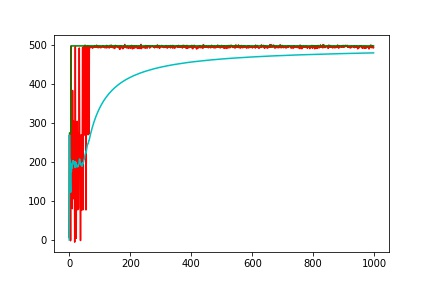
\includegraphics[scale=0.9]{grafi1.jpg}
  \caption[Primera ejecución]{Primera ejecución aproximando probabilidades}
  \label{graf1}
\end{figure}
\begin{figure}
  \centering
    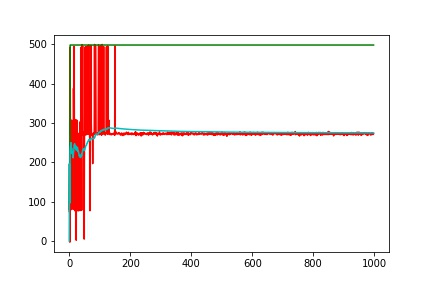
\includegraphics[scale=0.9]{grafi2.jpg}
  \caption[Segunda ejecución]{Segunda ejecución aproximando probabilidades}
  \label{graf2}
\end{figure}
\begin{figure}
  \centering
    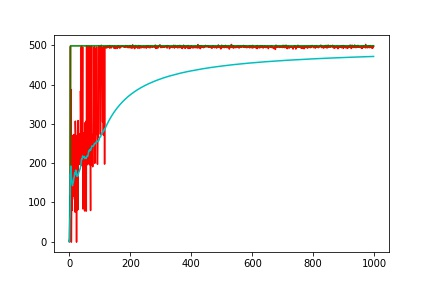
\includegraphics[scale=0.9]{grafi3.jpg}
  \caption[Tercera ejecución]{Tercera ejecución aproximando probabilidades}
  \label{graf3}
\end{figure}
\begin{figure}
  \centering
    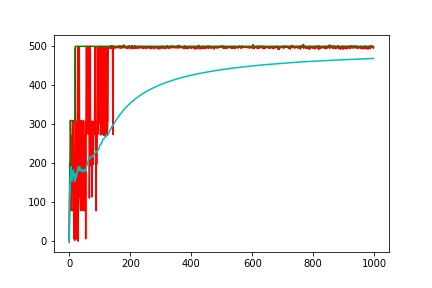
\includegraphics[scale=0.9]{grafi4.jpg}
  \caption[Cuarta ejecución]{Cuarta ejecución aproximando probabilidades}
  \label{graf4}
\end{figure}
\begin{figure}
  \centering
    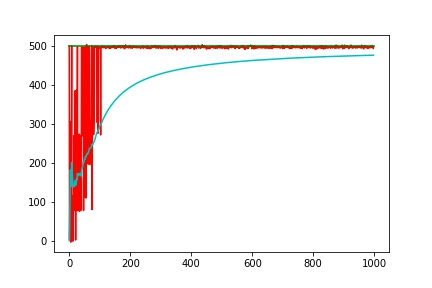
\includegraphics[scale=0.9]{grafi5.jpg}
  \caption[Quinta ejecución]{Quinta ejecución aproximando probabilidades}
  \label{graf5}
\end{figure}
\begin{figure}
  \centering
    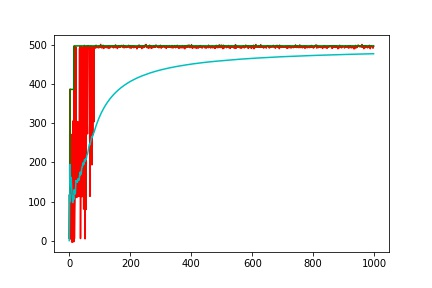
\includegraphics[scale=0.9]{grafi6.jpg}
  \caption[Sexta ejecución]{Sexta ejecución aproximando probabilidades}
  \label{graf6}
\end{figure}
\begin{figure}
  \centering
    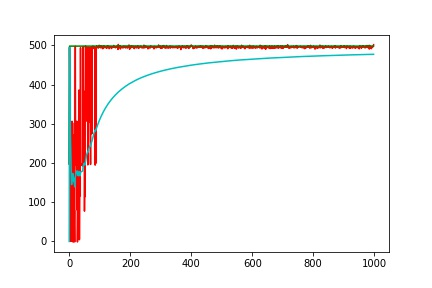
\includegraphics[scale=0.9]{grafi7.jpg}
  \caption[Séptima ejecución]{Séptima ejecución aproximando probabilidades}
  \label{graf7}
\end{figure}
\begin{figure}
  \centering
    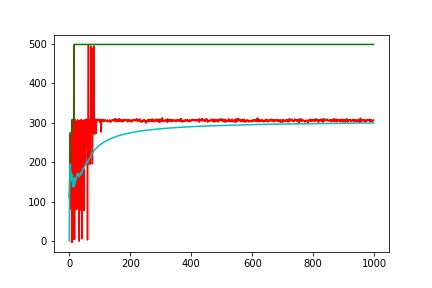
\includegraphics[scale=0.9]{grafi8.jpg}
  \caption[Octava ejecución]{Octava ejecución aproximando probabilidades}
  \label{graf8}
\end{figure}
\begin{figure}
  \centering
    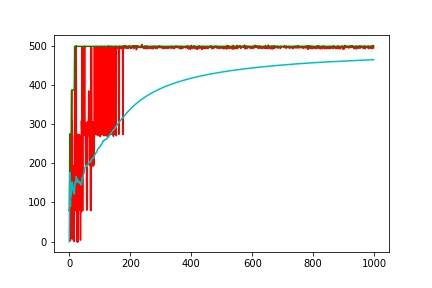
\includegraphics[scale=0.9]{grafi9.jpg}
  \caption[Novena ejecución]{Novena ejecución aproximando probabilidades}
  \label{graf9}
\end{figure}
\begin{figure}
  \centering
    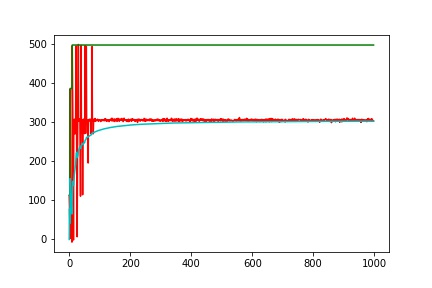
\includegraphics[scale=0.9]{grafi10.jpg}
  \caption[Décima ejecución]{Décima ejecución aproximando probabilidades}
  \label{graf10}
\end{figure}

De otra parte, en el anexo \ref{resultBandit10}, se aprecian los resultados de las 10 ejecuciones, todas con la respuesta correctas, junto con los arreglos donde, cada uno de los vectores que representa una ruta, hallada alguna vez por el algoritmo, tiene una ganancia promedio asociada y el número de veces que ha sido seleccionado.

No se presentan gráficas para mostrar la eficiencia de este aplicativo, puesto que no depende de alguna convergencia, sino que, únicamente, obedece a la fórmula de promedio de ganancias que ofrece el aprendizaje por refuerzo.
